\setlength{\columnsep}{3pt}
\begin{flushleft}
	
	\begin{figure}[h!]
		\centering
		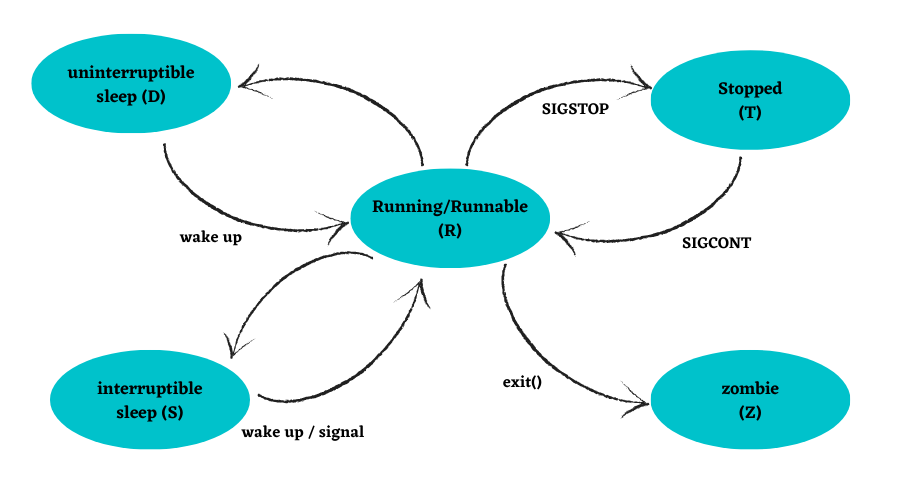
\includegraphics[scale=0.5]{content/chapter12/images/state_process.png}
		\caption{Process State}
		\label{fig:process_state}
	\end{figure}
	
	\begin{itemize}
		\item \textbf{Running}: 
		\begin{itemize}
			\item Process is either \textbf{running or ready to execute}.
			\item Denoted as \textbf{"R"}.
		\end{itemize}

		
		\bigskip
		\item \textbf{Interruptible sleep}: 
		\begin{itemize}
			\item Indicates the process is blocked.
			\item The process is waiting indirectly for some event.
			\item Eg: Some process is waiting for completion of an I/O operation.
			\item Denoted as \textbf{"S"}.
		\end{itemize}
		
		
		\bigskip
		\item \textbf{Uninterruptible sleep}: 
		\begin{itemize}
			\item Indicates the process is blocked.
			\item A process is waiting directly on hardware conditions.
			\item Eg: Printer running out of page.
			\item Denoted as \textbf{"D"}.
		\end{itemize} 
		
		\bigskip
		\item \textbf{Stopped}: 
		\begin{itemize}
			\item Halted process.
			\item Eg: A process that is being troubleshooted can be put into the stopped state.
			\item Denoted as \textbf{"T"}.
		\end{itemize}
		
		\bigskip
		\item \textbf{Dead}:
		\begin{itemize}
			\item Permanently stopped process.
			\item Dead process do not use RAM, CPU etc.
			\item Denoted as \textbf{"X"}.
		\end{itemize}
		
		
		\bigskip
		\item \textbf{Zombie}: 
		\begin{itemize}
			\item Zombie process are dead process but they still consume CPU \& RAM.
			\item Zombie process does not have process ID, but their process name is still present.
			\item They may result in CPU \& RAM wastage.
			\item Denoted as \textbf{"Z"}.
		\end{itemize}
		
	\end{itemize}


\end{flushleft}

\newpage


